\chapter{Event modelling}
\label{EventModelling}

\begin{flushright}{\slshape    
[Artefacts] mediate activity that connects a person not only with \\
 the world of objects, but also with other people. This means \\
that a person's activity assimilates the experience of humanity.} \\ \medskip
    ---  Aleksei N. Leontiev \cite{InteractionDe}, founder of activity theory
\end{flushright}

\marginpar{Parts of this chapter appear in \cite{Niezen2011}.}

Events are notable occurrences that can be associated with people, places and objects at a specific time instant, or during a specific time interval. In the previous chapter the modelling of objects and their capabilities was described. The focus of this chapter is on how the event and its associated time instant/interval can be modelled. The modelling of people and places is considered to be outside the scope of this thesis.

%- Event ontology
%- Music ontology (uses Events ontology, also see 15/02/11)

\marginpar{Interaction events were first introduced in Section \ref{OntologyDesign1}.}
% Interaction events are generated when a user interacts with a smart object. Interaction events are high-level input events which report the intention of the user's action directly, rather than just reporting the associated hardware input event that triggered the action.  

The W3C Web Events Working Group defined four conceptual layers for interactions, in the context of touch- and pen-tablet interaction \cite{w3cevents}:

\begin{description}
\item [Physical] This is the lowest layer, and deals with the physical actions that a user takes when interacting with a device, such as pressing a physical button.
\item [Gestural] This is layer describes mappings between the lower and upper layers; for example, a ``pinch'' gesture may represent the user placing two fingers on a screen and moving them together at the physical layer. This may map to a ``zoom-in'' event at the representational layer.
\item [Representational] This layer indicates the means by which the user is performing a task, such as zooming in, panning, navigating to the next page, activating a control, etc.
\item [Intentional] This layer indicates the intention of the task a user is trying to perform, such as viewing more or less detail (higher-level abstraction of zooming in and out), viewing another part of the larger picture (higher-level abstraction of panning), and so forth.
\end{description}

Interaction events can be defined at three of the layers, with the exception of the intentional layer. In Table \ref{transformationTable} examples of possible interaction events are shown, together with possible entities associated with these events. Most of these interaction events exist at the representational layer, which are events that have significant meaning. This high level of abstraction enables developers to write applications which will work across different devices and services, without having to write specific code for each possible input device.


\begin{table}
    \myfloatalign
  \begin{tabularx}{\textwidth}{ll} 
	\toprule
    \tableheadline{Interaction Event} & \tableheadline{Can be performed on } \\ 
    \midrule

	AdjustLevelEvent & Volume, Lighting \\
	switchOnEvent & Lighting, any SmartObject \\
	NavigateEvent & Playlist, Menu, SequentialData \\
	UndoEvent & Any other interaction event \\
	StopEvent & Application, Media \\
    \bottomrule
  \end{tabularx}
  \caption{Examples of interaction events in a smart environment}
\label{transformationTable}
\end{table}





%An interaction event has more than one possible entity that it can be performed on, as well as more than one possible entity that triggers it, i.e., there exists some ambiguity. Only when no ambiguity exists as to which entity it is performed on, as well as the action which the user is trying to accomplish, we refer to it as an intentional event. Semantic transformations occur between physical actions (such as pressing a button or doing a gesture) and representational events, as well as between representational events and intentional events.


%end S3E


These events all occur at a specific time or during a specific time interval. In \ac{OWL}, there are are two approaches to modelling time:

\begin{itemize}
	\item Using datatype properties -- event instances can be related to a literal with a \ac{XSD} datatype such as \texttt{xsd:date} or \texttt{xsd:dateTime}. %This is the approach that we used and is described later in this chapter.
	\item Using object properties -- classes are used to define temporal intervals, and event instances are linked to instances of these classes using object properties.
\end{itemize}

The advantage of linking event instances directly with dates is simplicity. There are fewer abstractions to deal with, and it is easier to sort events chronologically and compare them \cite{Shaw2009}. On the other hand, working with temporal intervals provide more flexibility and allows for more detailed temporal reasoning. 

This chapter is structured as follows: First we look at current approaches to modelling events using ontologies, which is then followed by our approach to modelling interaction events, based on the concepts of the existing event ontologies.
	%\item Categorising interaction events in terms of the layers of interaction described above 

\section{Related work}
We now look at various existing event ontologies that we build upon to model interaction events in ubiquitous computing environments. We will also look at how temporal reasoning is performed with ontologies.

\subsection{The Event Ontology}
The \ac{EO}\footnote{http://motools.sf.net/event/event.html} was developed within the context of the Music ontology\footnote{http://purl.org/ontology/mo/} at Queen Mary, University of London. Although originally created to describe musical performances and events, it is currently the most commonly used event ontology in the Linked Data community \cite{Shaw2009}.

The Timeline\footnote{http://motools.sf.net/timeline/timeline.html} ontology, used to define time instants and intervals, also forms part of this collection of ontologies. Reasoning with temporal information is discussed further in Section \ref{TemporalReasoning}.  

\subsection{DUL}

The \ac{DUL} upper ontology is a light\-weight version of the \ac{DOLCE} ontology. \ac{DUL} defines the class \texttt{Event} next to the disjoint upper classes \texttt{Object}, \texttt{Abstract} and \texttt{Quality} \cite{Scherp2011}. \ac{DUL} allows for both the approaches to modelling time with \ac{OWL}, either with the \texttt{hasEventDate} datatype property, or with a \texttt{TimeInterval} class and the \texttt{isObservableAt} object property.

Events can be related to a \texttt{Place} with the \texttt{hasLocation} property. Alternatively, events can be related to a \texttt{SpaceRegion} with the \texttt{hasRegion} property, where \texttt{Space\-Region} resolves to a geospatial coordinate system. \ac{DUL} uses a \texttt{hasParticipant} property to relate an event to an object, and uses the \texttt{hasPart} property to link events to sub-events.

\subsection{Event-Model-F}

The Event-Model-F ontology extends the \ac{DUL} ontology to describe events in more detail. To describe the participation of an object in an event, the Event-Model-F ontology uses the \ac{DnS} ontology design pattern \cite{Shaw2009}.\marginpar{The \ac{DnS} pattern is described in more detail in Chapter \ref{OntologyEngineering}.} 

An object is defined as a \texttt{Participant}, where \texttt{Lo\-ca\-tion\-Pa\-ra\-meter} is used to describe the general spatial region of the object \cite{Scherp2011}. \texttt{Time\-Parameter} describes the general temporal region when the event happened by parametrizing a \ac{DUL} \texttt{TimeInterval}. A composite event \texttt{Composite} is composed out of a number of \texttt{Com\-po\-nent}s.

\subsection{Linked Open Descriptions of Events (LODE)}

The \ac{LODE} ontology\footnote{http://linkedevents.org/ontology/} is an ontology for publishing descriptions of historical events as Linked Data. It builds upon the work of the previous ontologies described in this section, in order to improve interoperability with legacy event collections. Its \texttt{Event} class is directly equivalent to those defined by \ac{EO} and \ac{DUL}. 

It uses time intervals to link events to ranges of time, where its \texttt{atTime} property is a sub-property of the \ac{DUL} \texttt{isObservableAt} property. There is also a distinction between places and spaces, where the \texttt{inSpace} property relates the event to a space, and the \texttt{atPlace} property is a sub-property of the \ac{DUL} \texttt{hasLocation} property.


\subsection{Ontologies for temporal reasoning}
\label{TemporalReasoning}

Temporal reasoning is used when working with time intervals, for example when using Allen's Interval Algebra to define temporal relations between events. There are 13 base relations in this algebra, for example to define that event X happens before event Y, or that event X occurs during event Y. Allen's Interval Algebra is used by a number of ontologies, including the \ac{DOLCE} \cite{Scherp2011} upper ontology. \marginpar{The \ac{DOLCE} upper ontology is discussed in more detail in Chapter \ref{OntologyEngineering}.}

\ac{SWRL} Basic Temporal Built-ins support \texttt{xsd:date} and \texttt{xsd:\-date\-Time} with Allen's Interval Algebra. The Advanced Temporal Built-ins uses the \texttt{temporal} ontology \cite{OConnor2010} to provide additional functionality, for example having different granularity levels.


The \ac{DC} Terms ontology has a \texttt{temporal} property to describe temporal coverage of a resource with a range \texttt{periodOfTime}.

TopBraid Composer has a Calendar ontology that defines an \texttt{Event} and its \texttt{startTime} and \texttt{endTime} (as \texttt{xsd:dateTime}). This can then be used with the Calendar View widget in the editor. 

In \ac{SPARQL}, we can use the $<$ and $>$ operators on dates, for example 

\begin{verbatim}
FILTER(?date > "2005-10-20T15:31:30"^^xsd:dateTime)
\end{verbatim}

Using \ac{SPIN}, can also cast a \texttt{xsd:dateTime} value to a string using the \texttt{fn:substring} function, for example

\begin{verbatim}
fn:substring(xsd:string(afn:now()),0,10)
\end{verbatim}

We build on these event models to create our own interaction event model. In the next section, a mapping between the entities in the various ontologies show how our work relates to the existing work.


\section{Interaction events}
\label{InteractionEvents}

We now turn our focus to how interaction events are modelled in the work described in this thesis. In order to perform semantic reasoning with events, we need to know when they occur and be able to uniquely identify them. An interaction event happens at a specific time, is generated by a smart object and has an optional data value associated with the event.

\begin{figure}[bth]
        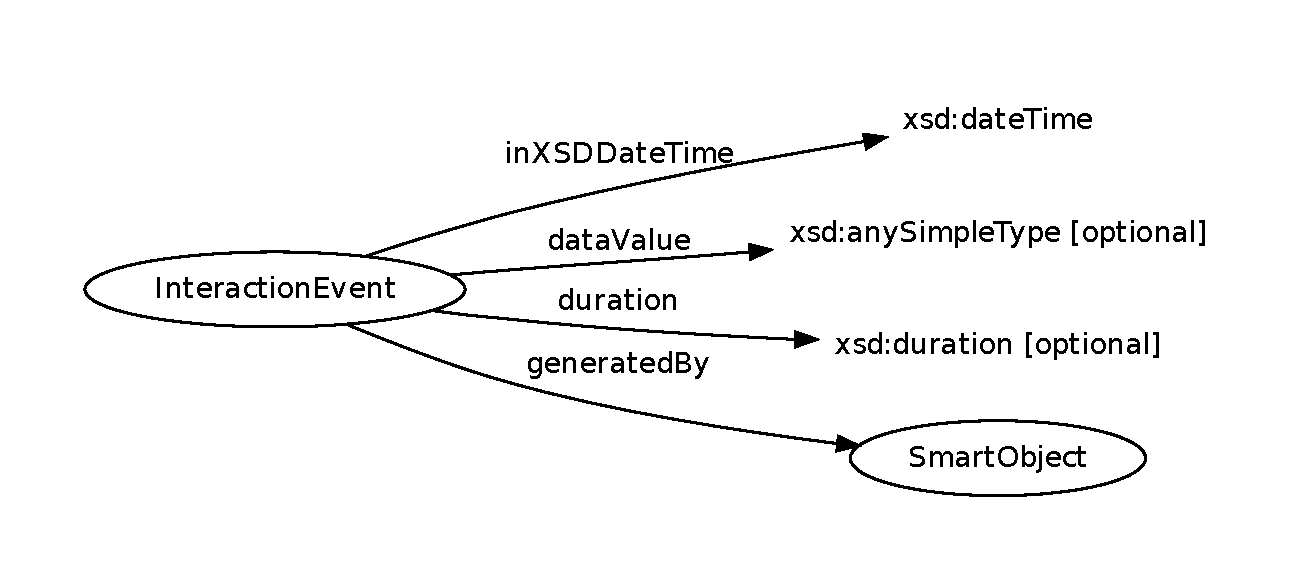
\includegraphics[width=\linewidth]{interactionEvent}
        \caption{An interaction event as modelled in the ontology}
        \label{interactionEvent}
\end{figure}

An example of an event generated when an alarm is set is
\begin{minted}{turtle}
:event-43495d51-29e3-11b2-807e-ac78eefc1f82 
  rdf:type :AlarmSetEvent ;
  :generatedBy :phone1 ;
  :inXSDDateTime "2012-01-17T11:22:06.887+01:00"^^xsd:dateTime ;
  :dataValue "2012-01-17T12:00:00+01:00"^^xsd:dateTime .
\end{minted}

A mapping between our interaction event model and the other event ontologies is shown in Table \ref{eventMappings}. Note that we do not model people or places in the current version of the ontology, as we consider these entities to be optional when describing interaction events.

\begin{table}
    \myfloatalign
  \begin{tabularx}{\textwidth}{llll} 
	\toprule
    \tableheadline{DUL} & \tableheadline{EO} & \tableheadline{LODE} & \tableheadline{Interaction Events}\\ 
    \midrule

isObservableAt & time & atTime & inXSDDateTime  \\
 & place & inSpace & \\
hasLocation & & atPlace & \\
hasParticipant & factor & involved & \\
involvesAgent & agent & involvedAgent & generatedBy \\
& & & dataValue \\	
    \bottomrule
  \end{tabularx}
  \caption{Mappings between the various event models (adapted from \cite{Shaw2009})}\label{eventMappings}
\end{table}



The \texttt{duration} property is used to define the length of event. For example to increase the brightness of a lamp, we can generate an event to increase a value to a set maximum over a time period:

\begin{minted}{turtle}
:event-43495d51-29e3-11b2-807e-ac78eefc1f83 
  rdf:type :IncreaseLevelEvent ;
  :generatedBy ie:wakeup1 ;
  :inXSDDateTime "2012-01-17T11:23:06.887+01:00"^^xsd:dateTime ;
  :dataValue 255 ;
  :duration "PT3S"^^xsd:duration .
\end{minted}


% We also distinguish between \emph{control} and \emph{content}. Interacting with a device, e.g. pressing a ``Play'' button or moving a volume slider, is considered control and described using interaction events. Content, e.g. a song or a photo stored on the device,  is referred to by where it exists on the device, as well as how it can be rendered using the media capabilities of the device. 

We consider interaction events to be identifiable and traceable. Each interaction event has an associated timestamp and a unique ID that is generated when the event occurs. All interaction events that occur are stored in the triple store.

\marginpar{Intentional, incidental and expected interactions were introduced in Section \ref{intentionalSpectrum}.}
An intentional interaction, like pressing a light switch, is an interaction event if the light switch shares this information with other devices. Incidental or expected interactions, like the light turning on if the presence sensor is triggered, are also interaction events. System events, like a \texttt{TimeSetEvent}, which are invisible to the user are not considered to be interaction events.

% \section{Categorising interaction events}
% 
% In the iStuff toolkit \cite{Ballagas2003} \emph{hierarchical event} structures were used to abstract low-level events into application-level events. \marginpar{Also see the related work on task models in Section \ref{interactionTasks}.} We also introduce the notion of an event hierarchy, where the designer of the smart object can specify at which level the event occurs. 
% 
% We build on the different interaction layers introduced in the related work of Section \ref{InteractionModels} to categorise interaction events. As an example, consider the case where a rocker switch, modelled as an interaction primitive on a mobile device, is used to control the volume of music in a room. One could start modelling the interaction on the physical level with a \texttt{ButtonEvent}, but it would be more meaningful to model it on the lexical level as a \texttt{ButtonUpEvent}. On the syntactic level this event could increment a quantity by one, while an event generated by a volume dial might have a discrete value attached to it. When this information is combined with other device information, for example that the device is being used to stream music to the environment, we can use semantic reasoning to infer on the semantic level that it is a \texttt{VolumeUpEvent}. When this is combined with other contextual information, for example that the device is currently connected to a speaker system in the same room, we can even infer on the task level that the music volume in the room should be set to a specific value with a \texttt{MusicVolumeUpEvent}, to which all connected devices can respond. We acknowledge that in most cases it may not be possible to make inferences on the goal level, which in this example could be the user's intent to set the music volume in the room to a level that is loud enough for everyone in the room to dance to.
% 
% \begin{figure}[bth]
% 	\digraph[scale=0.45]{InteractionModelToOntology}{
% 		{rank=same; Semantic [label="Semantic Level", shape=plaintext]; AdjustLevelEvent; MusicVolumeUpEvent }
% 		{rank=same; Syntactic [label="Syntactic Level", shape=plaintext]; VolumeUpEvent; SmartObject;}
% 		{rank=same; Lexical [label="Lexical Level", shape=plaintext]; ButtonUpEvent}
% 		{rank=same; Physical [label="Physical Level", shape=plaintext]; ButtonEvent; }
% 		Semantic->Syntactic->Lexical->Physical [style="invis"];
% 		ButtonEvent->ButtonUpEvent;
% 		ButtonUpEvent->VolumeUpEvent
% 		VolumeUpEvent -> MusicVolumeUpEvent;
% 		MusicVolumeUpEvent -> AdjustLevelEvent  [label="is-a"];
% 		VolumeUpEvent -> SmartObject [label="generatedBy"];
% 		AdjustLevelEvent -> SmartObject [label="generatedBy", style="dashed"];
% 	}
% 	\caption{How the interaction model levels relate to the ontology}
% 	\label{InteractionModelToOntology}        
% \end{figure}
% 
% Figure \ref{InteractionModelToOntology} shows how the interaction model levels relate to the concepts in the ontology that was developed through the various iterations. A \texttt{ButtonEvent} describes a user interaction on the physical level, but carries very little meaning. For example, was the button switched up or down, or was it pressed? If we know that the button was switched up, we have a lexical token that describes the interaction, but it still needs to be combined with other contextual information to determine the user's intention. On the other hand, if the interaction is described as a \texttt{VolumeEvent}, the user's intention is described on a syntactic level, and it becomes possible to map the event to a set of predefined semantic events, for example an \texttt{AdjustLevelEvent}. Using semantic reasoning, we can also infer that this \texttt{AdjustLevelEvent} was generated by the same smart object. Semantic reasoning is performed on the \ac{SIB}, so new events generated by different \acp{KP} may be used to recategorise existing events as more information becomes available.


\subsection{System events}
\label{SystemEvents}
When a smart object first subscribes to the smart space, it specifically listens for events that are generated by other smart objects connected to it. This means that we also need some way of distributing system-wide events that all devices listen for. As an example, consider the \texttt{TimeSetEvent}. When the user sets the time on one device, we want the time to be immediately updated on all the other smart objects in the smart space, even if they are not connected to the device that generated the \texttt{TimeSetEvent}. If we define \texttt{TimeSetEvents} as a subset of \texttt{SystemEvents}, each smart object only need to subscribe to events of type \texttt{SystemEvent}.


\subsection{Feedback}
When setting an alarm for example, augmented feedback should be provided on all devices. Functional feedback, i.e. the alarm sound when an alarm fires is triggered, is delayed. This means that augment functional feedforward should be provided. We thus define two types of feedback events:\marginpar{Preview events and indicator events were first introduced in Section \ref{section:augmentedFunctionalFf}.}

\begin{itemize}
\item \texttt{PreviewEvent} - generated when a possible connection is being explored, displaying the possible functionalities enabled by the connection, i.e. augmented functional feedforward.
\item \texttt{IndicatorEvent} - augmented feedback when smart object is connected and there is no immediate functional feedback, e.g. a sink ``beeping'' when the alarm is set on the source; used to confirm actions.   
\end{itemize} 

The type of feedback required depends on the functionality of the connection. It is important for the feedback to coincide in time and modality with the event generated, as to maintain the causal link that is perceived by the user.

The device used to make the connection, for example the Connector object, creates a temporary connection to the devices to be connected in order to generate a \texttt{PreviewEvent}. This \texttt{tempConnectedTo} property is a sub-property of the \texttt{connectedTo} property. This means that the smart objects will handle it as if it is a regular connection, and when the Connector object removes the \texttt{tempConnectedTo} relationship, the inferred \texttt{connectedTo} relationship will disappear as well.


\subsection{Discussion \& Conclusion}

\begin{figure}[bth]
	\begin{center}
        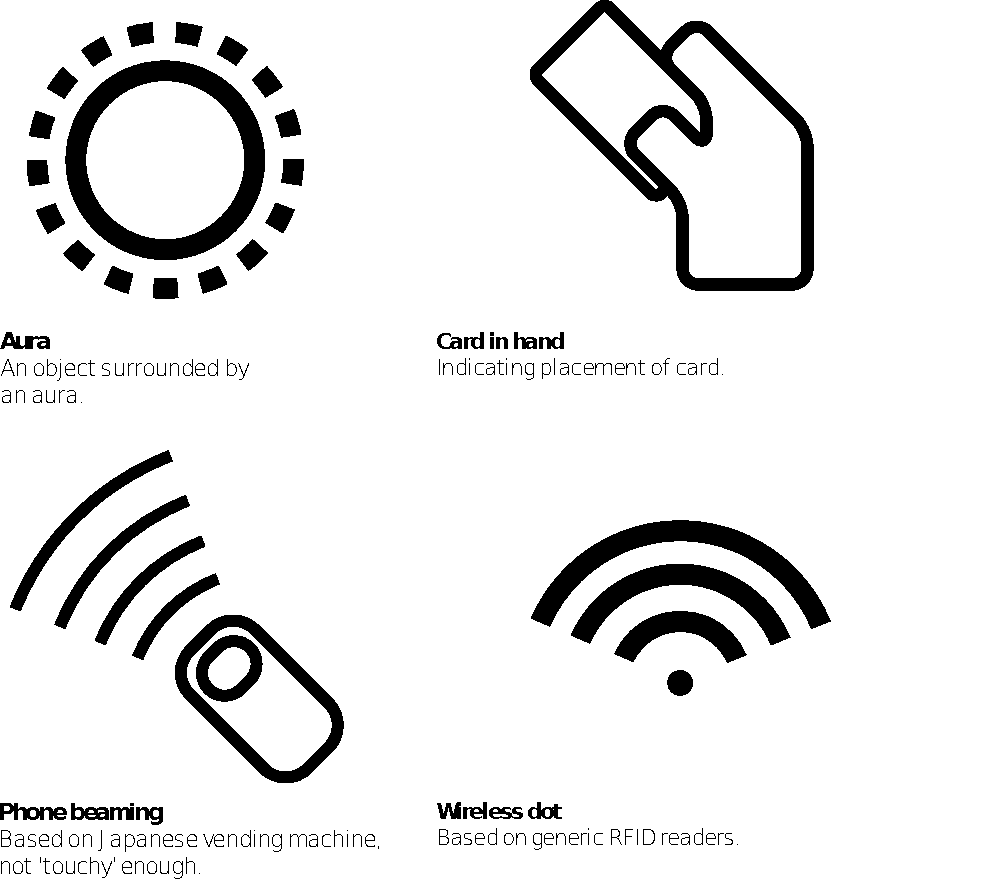
\includegraphics[width=250px]{arnall}
	\end{center}
        \caption{Examples from Arnall's ``A graphic language for touch'' (adapted from \cite{Arnall2006})}
        \label{arnall}
\end{figure}

Tungare et al. \cite{Tungare2007} defined a \emph{task disconnect} as ``the break in continuity that occurs due to the extra actions outside the task at hand that are necessary when a user attempts to accomplish a task using more than one device.'' Kuniavsky \cite{Kuniavsky} states that consistency is the key aspect in creating task continuity across devices, and that \emph{interaction vocabularies} have recently emerged as a way of consistently interacting with a range of devices. This ranges from simple vocabularies of light patterns and motion as used by the (now discontinued) Nabaztag Internet-connected rabbit that could compose ``sentences'' with more complex meaning, to a set of visual icons by Timo Arnall \cite{Arnall2006} that represents various kinds of touch-based RFID interactions.

These interaction vocabularies try to smooth over task disconnects through consistency. We argue that by having a vocabulary, or ontology, of interaction events could improve consistency in ubiquitous computing environments. This is the intention of the work in this chapter --- to provide an ontology of interaction events that improves consistency for users, as well interoperability between devices.

Arnall's touch-based vocabulary is shown in Figure \ref{arnall}. Arnall categorises his vocabulary of visual icons into four classes of interactions: 

\begin{itemize}
	\item Circles, of which the ``Aura'' is an example
	\item Card, of which the ``Card in hand'' is an example
	\item Wireless, of which the ``Wireless dot'' is an example
	\item Mobile, of which the ``Phone beaming'' is an example
\end{itemize}


The ``Aura'' icon communicates both the near-field communication capabilities of the technology, but also indicates that the physical object has capabilities beyond its form. The icons with cards or mobiles could improve consistency for a wide range of users which use these technologies on a daily basis.

Arnall's work is specific to touch-based RFID interactions, and helps to provide users with feedforward of device functionality that might not be immediately apparent otherwise. An ontology of interaction events, on the other hand, provides designers of smart objects with a vocabulary to describe the events that are shared between devices in order to improve interoperability and consistency.





% TODO: Valkkynen2010,  Rekimoto et al. (Ayatsuka2003), Nordby2010

% http://www.elasticspace.com/presentations/graphic_language_touch_rfid_nfc.pdf

% Possible TODO: How we developed a vocabulary for semantic connections

% Possible TODO: Creating a vocabulary of interaction events (based on existing task models)



% ===Event modelling
% To model an \texttt{AlarmSetEvent}, the following restriction was used:\\
% 
% \noindent
% \texttt{AlarmSetEvent}~$\models$~\texttt{SetEvent}~$\sqcap$~\texttt{dataValue}~$\forall$~\texttt{xsd:dateTime}~$\sqcap$~\texttt{dataValue}~$= 1$\\
% 
% This restriction will not infer that an event is an \texttt{AlarmSetEvent}, but it will restrict the descriptions of these events to what can actually be described.
